\authoredSection{corny}{Toolchain}
Im Rahmen unseres Projekts wurde uns schnell klar, dass wir auf viele Tools angewiesen sein würden. So musste unser Quelltext versioniert, die grobe Struktur und Views festgehalten und Aufgabenpakete erstellt und koordiniert werden. Darüber hinaus war uns auch Design und Qualität wichtig. Auf unsere Erfahrungen in diesem Zusammenhang gehen wir im folgenden Abschnitt ein.

\subsection{Versionsverwaltung und Informationsaustausch}
	Um kollaborativ an einer Software zu arbeiten ist es selbstverständlich erforderlich, mit Quelltextversionierung zu arbeiten. Da bei uns Team-Mitgliedern die Erfahrung mit Git \cite{Git14} aus dem Universitäts- und Arbeitsumfeld am größten war, viel unsere Wahl für ein \acs{VCS} darauf.
	
\begin{figure}[h!]
	\centering
	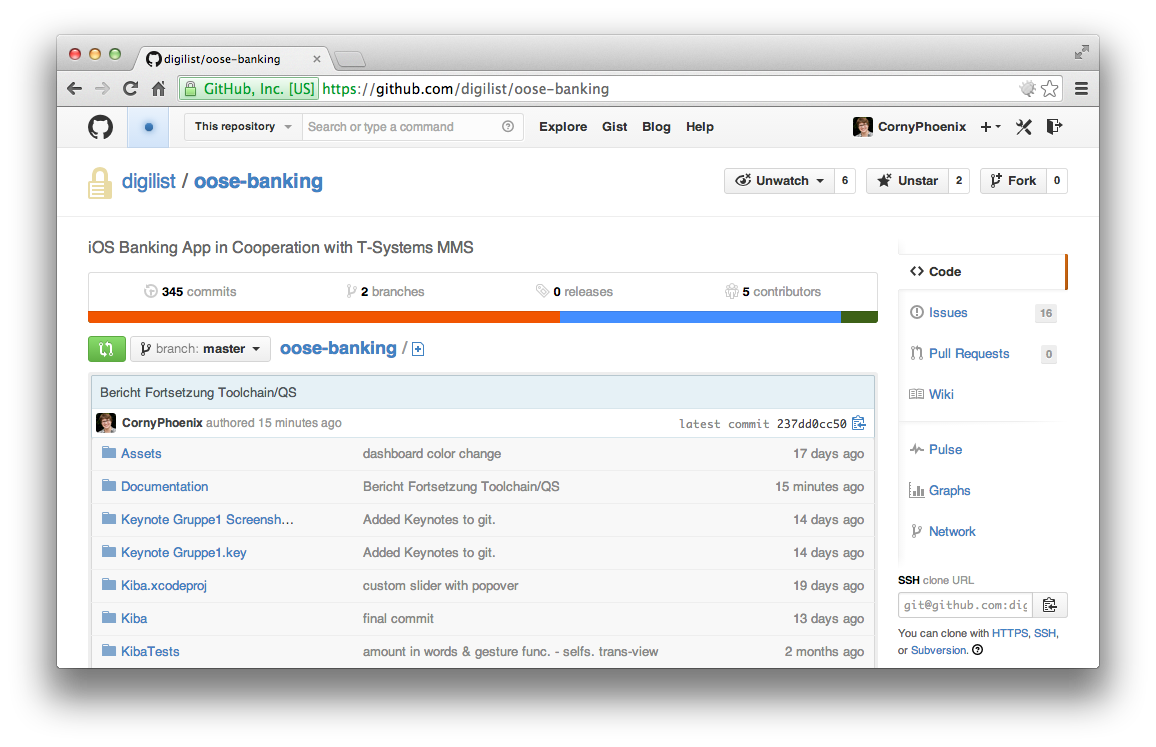
\includegraphics[scale=.25]{Pictures/GitHubOverview}
	\caption{Repository-Hosting bei GitHub \label{fig:GitHubOverview}}
\end{figure}
	
	Entscheidend dabei war auch der größere Komfort gegenüber Subversion. Einerseits ist die operative Geschwindigkeit von Git deutlich schneller \cite{svngit}, sorgt also im Team für eine Produktivitätssteigerung. Dieser Punkt ist in sofern für und von Relevanz, als dass auch wir ein Problem mit größeren Dateien, wie den XIB-Views, hatten. Auf der anderen Seite erlaubt Git durch sein verteiltes System Branches pro Anwender zu führen, wodurch auch ermöglicht wird, Commits  unabhängig vom Internet zu publizieren. 
	
	Darüber hinaus schuf Git auch die Möglichkeit, die eng verwandte Plattform „GitHub“ \cite{GitHub14} als Repository-Hoster zu verwenden. Dieser bietet über den für die Versionsverwaltung erforderlichen Speicherplatz hinaus auch eine sehr gute grafische Bedienoberfläche, wie sie in Abbildung \ref{fig:GitHubOverview} zu sehen ist.
	
	Ein weiteres nützliches Feature von GitHub für uns war außerdem das zuvor erwähnte Wiki, dargestellt in Abbildung \ref{fig:WikiHome}. Ein Wiki hatte für uns den Vorteil eines demokratischen Informationsaustauschs; jeder konnte seine Erfahrung mit anderen Projektmitgliedern teilen, sodass alle davon profitierten. Daher tauschten wir in ihm erste Feature-Ideen oder auch Kontaktdaten aller Mitglieder aus. Allerdings nutzten wir es darüber hinaus auch für das Festlegen eines Arbeitsablaufs mit Xcode, ins Besondere das Code Styling oder das Verwenden bestimmter Plugins.

\subsection{Issue-Tracking-System}
	Da uns freundlicherweise von C1 WPS die Möglichkeit gegeben wurde, eine Scrum-Zer\-ti\-fi\-zie\-rung zu erhalten, lag uns viel daran, den Scrum-Ansatz so gut es ging in unseren Projekt-Ablauf zu integrieren. Dementsprechend war für uns bei der Frage nach einer unterstützenden Software wichtig, inwiefern es Scrum-Iterationen unterstützt und erleichtert.
	
\begin{figure}[h]
	\centering
	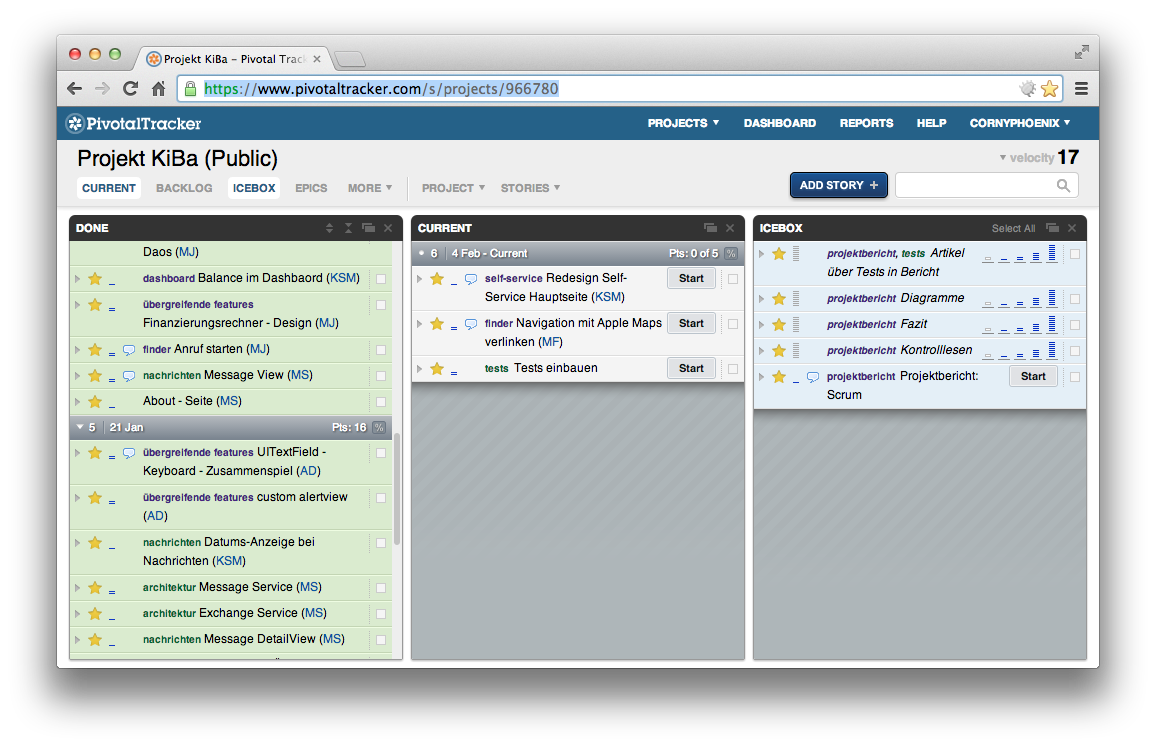
\includegraphics[scale=.25]{Pictures/TrackerStories}
	\vspace{-.8cm}
	\caption{Stories in PivotalTracker\label{fig:TrackerStories}}
\end{figure}
	
	Dazu verwendeten wir – nach ersten Versuchen mit GitHub-Issues – die Software PivotalTracker. Mit ihr können wir, wie in Abbildung \ref{fig:TrackerStories} dargestellt, einzelne Stories erstellen und überwachen. Ein großer Vorteil dabei war, dass Scrum-Iterationen automatisch von der Software generiert werden, berechnet durch unsere durchschnittliche Arbeitskraft (genannt „Velocity“)\footnote{\url{http://www.pivotaltracker.com/community/tracker-blog/velocity-matters}, Abruf 23.02.2014 um 18:00 Uhr.} und unseren Vorhersagen für den Aufwand einer Story angegeben durch Punkte.

	Zum anderen generiert PivotalTracker auch Burndown-Charts, welche für das Vorgehen während der Scrum-Iterationen unabdinglich sind. Denn so können wir am besten den Fortschritt unserer App messen und haben ein Monitoring für das Fortschreiten der Entwicklung unserer Features zu sehen ist.

\subsection{Konzept- und Designwerkzeuge}
\begin{figure}[hb]
	\centering
	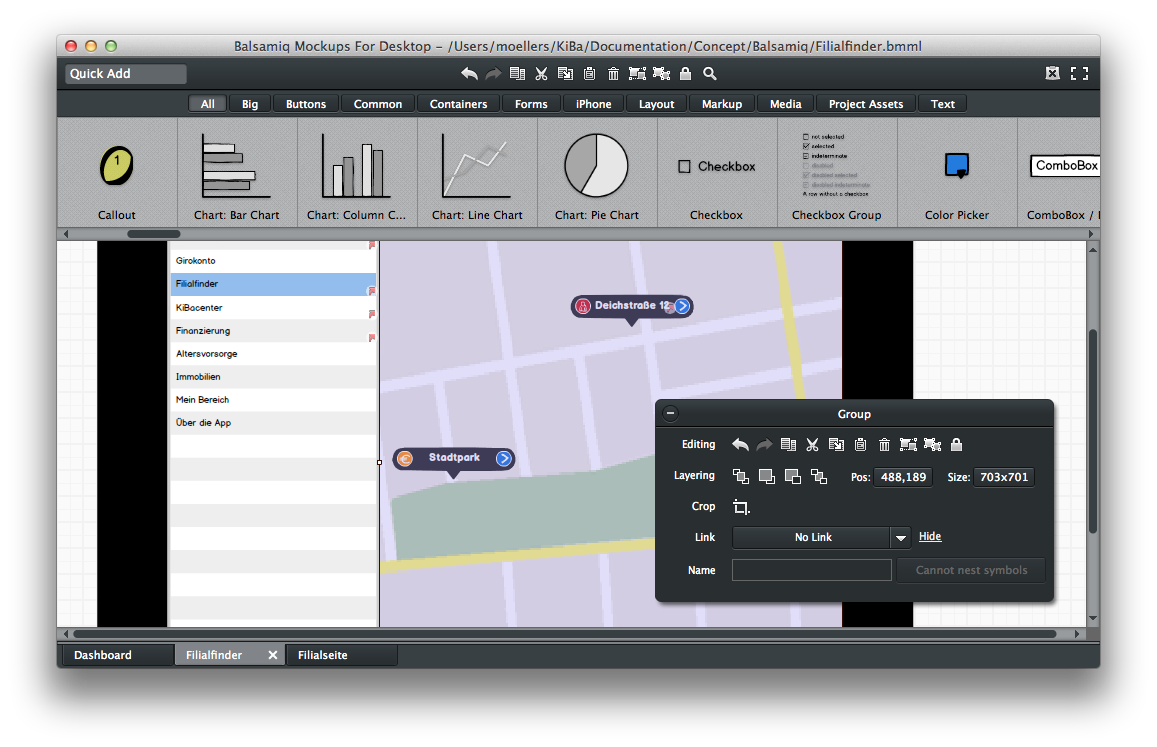
\includegraphics[scale=.3]{Pictures/BalsamiqEntwurf}
	\vspace{-.8cm}
	\caption{Mockup-Entwurf mit Balsamiq\label{fig:BalsamiqEntwurf}}
\end{figure}
	
	Für das Anfertigen von qualitativen Mockups, die für eine zielführende Implementierung von besonderer Bedeutsamkeit sein können, benötigt man Software, die einem in diesem Vorhaben gut unterstützt.
	
	Mit der in Abbildung \ref{fig:BalsamiqEntwurf} dargestellten Software „Balsamiq“\footnote{\url{http://balsamiq.com/}, Abruf am 23.02.2014 um 18:50 Uhr.}, die auch in einem Seminar der T-Systems MMS angesprochen wurde, fanden wir eine gute Lösung. Das interne Asset-Management ermöglicht es, Grafiken, die in diversen Mockups benötigt werden, auszutauschen und zu konservieren. Eine weitere nützliche Funktionalität stellte das Verknüpfen von Mockups da, womit man klickbare Referenzen zwischen den Dokumenten herstellt und in einer einfachen Simulation einen Eindruck von der Bedienbarkeit der finalen Version bekommt.

\begin{figure}[hb]
	\centering
	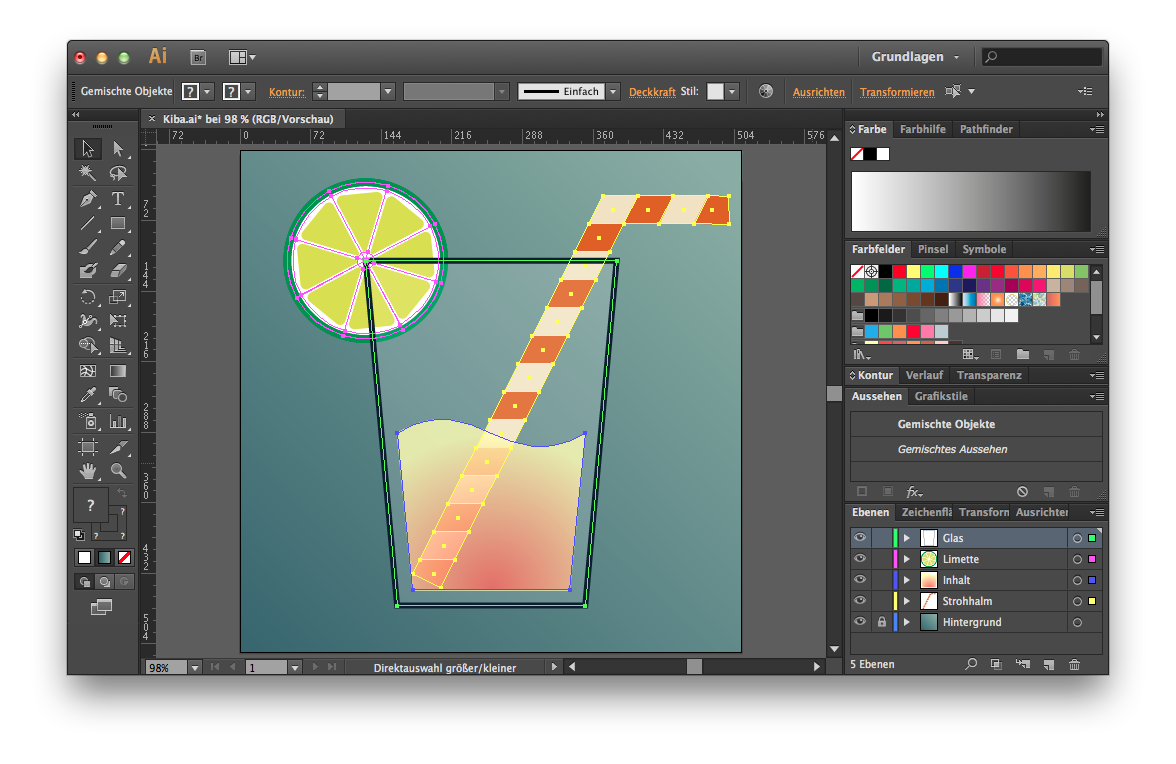
\includegraphics[scale=.3]{Pictures/IllustratorIcon}
	\vspace{-.8cm}
	\caption{Designen des KiBa-Icons mit Adobe Illustrator\label{fig:IllustratorIcon}}
\end{figure}

	Zuletzt, für das Finalisieren von Grafiken und Inhalten, waren auch Adobe Illustrator und Photoshop von großer Bedeutung für uns. Wenn es beispielsweise um die Bearbeitung des Icons geht, welche in Abbildung \ref{fig:IllustratorIcon} ersichtlich ist, wären frei verfügbare Bibliotheken für unsere Zwecke am Ende nicht mehr ausreichend. Daher haben wir auf qualitative Eigenproduktionen gesetzt.
